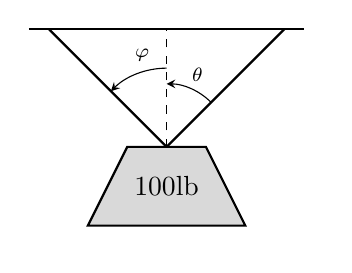
\begin{tikzpicture}
	
	\filldraw[thick,black,fill=gray!30] (-.5,0) -- (.5,0) -- (1,-1) -- (-1,-1)--cycle;
	\draw (0,-.5) node {100lb};
	
	\draw [thick] (-1.75,1.5) -- (1.75,1.5);
	\clip (-1.5,1.5) rectangle (2,-1.25);
	\draw [thick,rotate=135] (0,0) -- (3,0);% node[below,sloped,pos=.5] {\scriptsize $\vec F_2$};
	\draw [thick,rotate=45] (0,0) -- (3,0); %node[below,sloped,pos=.5] {\scriptsize $\vec F_1$};;
	\draw [dashed] (0,0) -- (0,2);
	\draw [rotate=45,->,>=stealth] (.8,0) arc (0:45:.8);
	\draw [rotate=67] (1,0) node {\scriptsize $\theta$};
	\draw [rotate=90,->,>=stealth] (1,0) arc (0:45:1);
	\draw [rotate=105] (1.2,0) node {\scriptsize $\varphi$};
	%\draw [dashed] (-1.5,0) -- (2,0);
	%\draw [dashed,->,>=stealth] (.6,0) arc (0:120:.6);
	%\draw [rotate=20] (.9,0) node {\scriptsize $120^\circ$};
	%\draw [dashed,->,>=stealth] (1.5,0) arc (0:45:1.5);
	%\draw [rotate=15] (1.8,0) node {\scriptsize $45^\circ$};

	
\end{tikzpicture}
